

\section{Thermodynamics and Statistical Mechanics}
(such as the laws of thermodynamics, thermodynamic
processes, equations of state,
ideal gases, kinetic theory, ensembles,
statistical concepts and calculation of
thermodynamic quantities, thermal
expansion and heat transfer)

\subsection{Laws of Thermodynamics}
\center
\begin{tabular}{|c|p{12 cm}|}
\hline

Zeroth Law & If two systems are in thermal equilibrium independently with a third system, they must be in thermal equilibrium with each other. This law helps define the notion of temperature.
 
\\ \hline

First Law & When energy passes, as work, as heat, or with matter, into or out from a system, its internal energy changes in accord with the law of conservation of energy. Equivalently, perpetual motion machines of the first kind are impossible.

$\Delta U = Q + W$
  
 \\ \hline
 
\end{tabular}
\flushleft

\center
\begin{tabular}{|c|p{12 cm}|}
\hline

Second Law &  In a natural thermodynamic process, the sum of the entropies of the interacting thermodynamic systems increases. Equivalently, perpetual motion machines of the second kind are impossible.
  
\\ \hline

Third Law & The entropy of a system approaches a constant value as the temperature approaches absolute zero. With the exception of non-crystalline solids (glasses) the entropy of a system at absolute zero is typically close to zero, and is equal to the logarithm of the multiplicity of the quantum ground states.
 
 \\ \hline
 
\end{tabular}
\flushleft

\center
\begin{tabular}{|c|c|}
\hline
 Fundamental Assumption & In an isolated system, all accessible microstates are equally probable.
 
 \\ \hline

\end{tabular}
\flushleft


%%%%%%%%%%%%%%%%%%%%%%%%%%%%

\subsection{Thermodynamic Processes}
\Table{
\hline

$W$ for an ideal gas & $W = - \int\limits_{V_i}^{V_f}p\,dV$

\\ \hline

$W$ in a $PV$ diagram is ... & ... area under the curve.

\\ \hline
}

%%%%

\Table{
\hline

\bf{Isothermal} & Constant temperature!

\\ \hline

$constant = $ & $PV = constant$

\\ \hline

$W = $ & $W = nRT\ln \Big[\dfrac{V_f}{V_i}\Big]$

\\ \hline

Internal energy ... & ... does not change. (Equipartition Theorem)

\\ \hline
}

%%%%

\Table{
\hline

\bf{Adiabatic} & No heat gained or lost by the system.

\\ \hline

$constant = $ & $PV^\gamma = constant$

\\ \hline

$\gamma = $ & $\dfrac{C_P}{C_V} = \dfrac{f+2}{f}$

 \\ \hline
 
 $W$ & $W =PV^\gamma \dfrac{V_f^{1-\gamma} - V_i^{1-\gamma}}{1-\gamma}$

 \\ \hline
}

%%%%

\Table{
\hline
 
 Adiabat or isotherm steeper in $PV$? & Adiabatic

\\ \hline

$W, Q, \Delta U$  for adiabatic free expansion & $W=0 \,, Q=0 \,, \Delta U = 0$

\\ \hline

Critical point & $\Big(\dfrac{\partial p}{\partial V} \Big)_T = \Big(\dfrac{\partial^2 p}{\partial V^2} \Big)_T = 0$

 \\ \hline
}

\Table{
\hline
\MiniPg{.2}{

Liquid-vapor phase diagram PV

}

&

\MiniPg{.8}{
\GraphicWHN{1}{.5}{PhasePV.png}
\tiny \url{http://cnx.org/contents/0zRIzO8t@1/13-6-Phase-Changes}
}

\\ \hline
}

%%%%

\Table{
\hline
\MiniPg{.2}{

H$_2$O phase diagram PT

}

&

\MiniPg{.8}{
\GraphicWHN{.6}{.5}{h2oPT.jpg}
\tiny \url{http://cnx.org/contents/0zRIzO8t@1/13-6-Phase-Changes}
}
\\ \hline
}

%%%%

\Table{
\hline

Fourier's law

&
\MiniPg{.7}{
\center
$\vv{q} = - k \nabla T$, where 

$\vv{q}$ is the local heat flux density, W$\cdot$m$^{-2}$,

$k$ is the material's conductivity, W$\cdot$m$^{-1}$K$^{-1}$

$\nabla T$ is the temperature gradient, K$\cdot$m$^{-1}$.
}

\\ \hline
}

%%%%%%%%%%%%%%%%%%%%%%%%%%%%%%%%

\subsection{Thermal expansion and heat transfer} 
\Table{
\hline

Heat capacity & $C = \dfrac{Q}{\Delta T}$

 \\ \hline

Specific heat capcacity & $c = \dfrac{C}{m} \rightarrow Q = mc \Delta T$
 
 \\ \hline

Latent heat & $L = Q/m$

 \\ \hline
}

%%%%%%%%%%%%%%%%%%%%%%%%%%%%%%%%%%%%%%%%%%%



\subsection{Engines \& Refrigerators}
\Table{
\hline

CW and CCW & Engines: CW. Fridges: CCW. \\
			& Think at const. $V$ what happens, $P \uparrow \downarrow$?

\\ \hline
}

%%%%

\Table{
\hline

Engine efficiency & $\eta = \dfrac{W}{Q_H} = 1 - \dfrac{Q_C}{Q_H} $

\\ \hline

Refrigerator Coefficient of performance & $\textrm{CP}_R = \eta_R = \dfrac{Q_C}{W} = \dfrac{Q_C}{Q_H - Q_C} $ 

\\ \hline

Heat pump efficiency & $\textrm{CP}_H = \eta_H = \dfrac{Q_H}{W} = \dfrac{Q_H}{Q_H - Q_C} $

\\ \hline
}

%%%%

\Table{
\hline

Carnot cycle is ... & Adiabat, Isotherm, Adiabat, Isotherm

\\ \hline

Carnot entropy & $dS = \dfrac{dQ}{T} = 0$ (Carnot)

\\ \hline
}

%%%%

\Table{
\hline

Heat entering system along isotherm & $Q = nRT\ln\Big(\dfrac{V_{end}}{V_{start}} \Big)$

\\ \hline
}

%%%%

\Table{
\hline

Carnot engine efficiency & $\eta = 1-\dfrac{T_C}{T_H}$ (Carnot)

\\ \hline

Carnot refrigerator efficiency & $ \textrm{CP}_R = \eta_R  = \dfrac{T_C}{T_H - T_C} $ (Carnot)

\\ \hline

Heat pump efficiency & $\textrm{CP}_H = \eta_H =  \dfrac{T_H}{T_H - T_C} $ (Carnot)

\\ \hline
}


%%%%%%%%%%%%%%%%%%%%%%%%%%%%%%%%%%%%%%



\subsection{Equations of state} 
\Table{
\hline

Thermodynamic identity & $dU = T\,dS- p\,dV + \mu\,dN$

\\ \hline

Change in entropy & $\Delta S \geq \frac{Q}{T}$, const. $T$, no spontaneous $\Delta S$

\\ \hline
}

%%%%

\Table{
\hline

Helmholtz Free Energy & $F = U - TS$ @ const. $T$ \\
				& $F_{sys} = $ min when $S_{universe} = $ max.

\\ \hline

Gibb's Free Energy & $G = U - TS + PV$

\\ \hline
}

%%%%

\Table{
\hline

Definition of Entropy & $S = k \ln \Omega$

\\ \hline

Definition of Temperature & $\dfrac{1}{T} = \Big( \dfrac{\partial S}{\partial U} \Big)_{V,N} $

\\ \hline
}

%%%%

\Table{
\hline

Chemical potential & $\mu = -T \Big(\dfrac{\partial S}{\partial N}\Big)_{U,V}$ \\
			& also $\mu = \Big(\dfrac{\partial U}{\partial N}\Big)_{S,V}$ \\
			& also $\mu = \Big(\dfrac{\partial F}{\partial N}\Big)_{T,V}$

\\ \hline
}

%%%%

\Table{
\hline

For systems $A$ and $B$ in diffusive contact & $A \rightarrow B$ \\ 
with $\mu_A > \mu_B$, which way do particles flow? &

\\ \hline
}

%%%%

\Table{
\hline

Heat capacity, constant volume

&

$C_V = \BigP{\dfrac{\partial E}{\partial T}}_V$

\\ \hline

Heat capacity, constant pressure

&

$C_P = \BigP{\dfrac{d E}{d T}}_P + P\BigP{\dfrac{d V}{dT}}_P$

\\ \hline
}

%%%%%%%%%%%%%%%%%%%%%%%%%%%%%%%%


\subsection{Ideal gases} 
\Table{
\hline

Ideal gas law & $PV=nRT=NkT$

\\ \hline

Relation between &  $nR$ is the number of moles times the Gas Constant.\\
 $n,N,k$ and $R$ & $Nk$ is the number of molecules times the Boltzmann Constant.
 
 \\ \hline
}

%%%%

\Table{
\hline
 
 $k=$ & $1.38 \times 10^{-23} \textrm{ J/K}$
 
 \\ \hline
 
 $R = $ & $k N_A = 1.38 \times 10^{-23} \textrm{ J/K} \, \times \, 
 6.02 \times 10^{23} \textrm{ mol}^{-1} = 8.31 \textrm{ J mol$^{-1}$ K$^{-1}$ }$
 
 \\ \hline
}

%%%%

\Table{
\hline
 
 Multiplicity of an IG & $\Omega(N,V,U) = f(N)\,V^N\,U^{fN/2}$ 
 
 \\ \hline
}

%%%%

\Table{
\hline

\MiniPg{.4}{Standard Temperature and Pressure}

&

\MiniPg{.6}{
\center
Standard Temperature = $0^{\circ} $ C $ = 273.15 $ K

Standard Pressure $1 $ Atm $= 101.3$ kPa.

1 mole of gas occupies 22.4 L.

}

\\ \hline
}


%%%%%%%%%%%%%%%%%%%%%%%%%%%%%%


\subsection{Kinetic theory} 
\Table{
\hline

Equipartition Theorem & $U = \dfrac{f}{2}NkT$

\\ \hline

$v_{rms} $ & $= \sqrt{\bar v^2} = \sqrt{\dfrac{v_1^2 + v^2_2 + ... + v^2_N}{N}}$

\\ \hline

$\dfrac{1}{2}m \bar v^2 =$ & $ \dfrac{3}{2}kT$

\\ \hline
}

%%%%

\Table{
\hline

Mean free path & $l = \dfrac{1}{n \sigma}$ where $n$ is number density $\dfrac{N}{V}$.

\\ \hline

$L_{rms} $&  $\sqrt{N}\,l$

 \\ \hline
 
 Distance between particles & $d = \Big( \dfrac{V}{N} \Big)^{1/3}$
 
 
\\ \hline
}

%%%%

\Table{
\hline
Degrees of freedom

&
\begin{minipage}{.75\textwidth}

      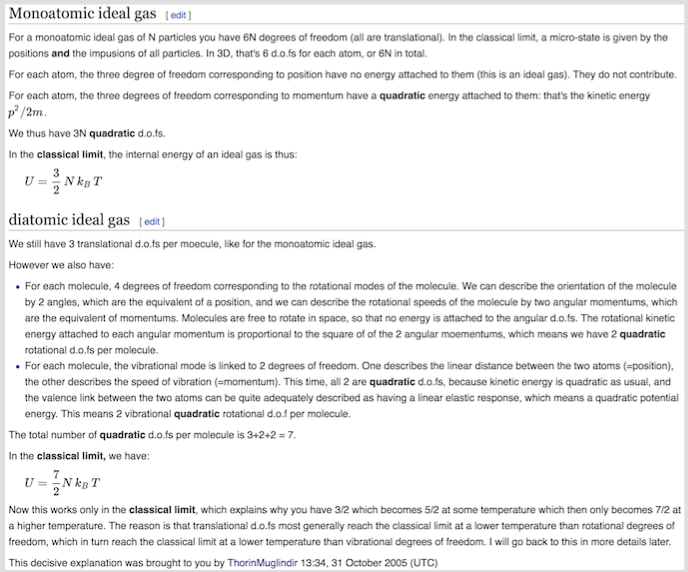
\includegraphics[width=\linewidth, height=130mm]{images/DOFs.png}

\tiny \url{https://en.wikipedia.org/wiki/Talk\%3ADegrees_of_freedom_(physics_and_chemistry)}

\tiny \url{http://demonstrations.wolfram.com/TheSixDegreesOfFreedomOfADiatomicMolecule/}
\end{minipage}

\\ \hline
}


%%%%%%%%%%%%%%%%%%%%%%%%%%%%%%%%%%%%%


\subsection{Ensembles} 
\Table{
\hline

Fermi energy & 
\begin{minipage}{.7\textwidth}
the energy difference between the highest and lowest occupied single-particle states in a quantum system of non-interacting fermions at absolute zero temperature
\end{minipage}

\\ \hline
}

%%%%

\Table{
\hline

\begin{minipage}{.3\textwidth}
Fermi Energy of infinite square well with N atoms
\end{minipage}
&
\begin{minipage}{.7\textwidth}
$E_F = \dfrac{\hbar^2 \pi^2}{2 m L^2}(N/2)^2$ for even $N$, and for odd $N$ substitue $N-1$ for $N$ in the expression.
\end{minipage}

\\ \hline
}

%%%%

\Table{
\hline

\begin{minipage}{.3\textwidth}
Fermi energy of a metal with $N$ electrons per volume $V$
\end{minipage}
&
\begin{minipage}{.7\textwidth}
\center
Metal $\approx$ 3-D ISW

$E_{n_x,n_y,n_z} = E_0 + \dfrac{\hbar^2 \pi^2}{2mL^2}(n_x^2 + n_y^2 + n_z^2)$,

but let $\vv{n} = \{n_x,n_y,n_z\}$ so that

$E_{\vv{n}} = E_0 + \dfrac{\hbar^2 \pi^2}{2mL^2}|\vv{n}|^2$.

In the ground state, the number of fermions is

$N = 2 \times \dfrac{1}{8} \times \dfrac{4}{3}\pi n_F^3$ where $|n_F|$ is the radius of the Fermi-sphere in $n$-space. Thus,

$n_F = \Big(\dfrac{3N}{\pi}\Big)^{1/3}$.

So, the Fermi energy is

$E_F = \dfrac{\hbar^2 \pi^2}{2mL^2}n_F^2 = \dfrac{\hbar^2 \pi^2}{2mL^2}\Big(\dfrac{3N}{\pi}\Big)^{2/3}$

$\boxed{E_F = \dfrac{\hbar^2}{2m}\Big(\dfrac{3\pi^2N}{V}\Big)^{2/3} }$

\end{minipage}

\\ \hline
}

%%%%

\Table{
\hline

\begin{minipage}{.3\textwidth}
Fermi temperature, momentum, velocity and wave vector
\end{minipage}
 &
\begin{minipage}{.7\textwidth} 
  $T_F = \dfrac{E_F}{k_B}$; \; \; \;  $p_F = \sqrt{2m_eE_F}$; \; \; \; $v_F = \dfrac{p_F}{m_e}$; \; \; \; $k_F = \dfrac{p_F}{\hbar}$
\end{minipage}

\\ \hline

typical Fermi energy for metal & $10^{28}$ to  $10^{29}$ e/m$^3$ $\rightarrow E_F \approx 2 $ to $ 10$ eV

\\ \hline
}


%%%%
\Table{
\hline

\begin{minipage}{.3\textwidth}
Number of independent oscillators in crystal with $N$ atoms 
\end{minipage}
& $3N$ according to Einstein and Debye

\\ \hline
}

%%%%

\Table{
\hline

Multiplicity of an Einstein Solid & $\Omega = {{q+N-1}\choose{q}} = \dfrac{(q+N-1)!}{q!\, (1 +N-1 - q)!}$ \\

& $ = \dfrac{(q+N-1)(q + N - 2) ... (q + N - q) (N - 1) (N-2) ...}{q!  (N - 1) (N-2) ...}$ \\

& $ = \dfrac{(q+N-1)(q + N - 2) ... N}{q!}$

\\ \hline
}

%%%%

\Table{
\hline

Entropy of an Einstein Solid & $S = k (\ln (1 + N)! - \ln q! - \ln N!)$ \\
 & Stirling's $\rightarrow$ \\
 & $\ln \Omega \approx (q + N) \ln(q + N) - (q+ N) - q \ln q + q - N \ln N + N$ \\
 & $=(q+N) \ln(q + N) - q \ln q - N \ln N $ \\
 & ... and ...\\
 & $\ln(q + N) = \ln \Big[q\Big(1 + \dfrac{N}{q} \Big) \Big]$ \\
 & $ = \ln q + \ln \Big( 1 + \dfrac{N}{q} \Big)$ \\ 
 & $ \approx \ln q + \dfrac{N}{q}$  assuming $q>>N$\\
 & ... algebra ... \\
 & $S = k \ln \Omega = k \Big( N \ln \dfrac{q}{N} + N + \dfrac{N^2}{q}\Big) $ \\
 & drop the last term \\
 & $S \approx Nk\Big(\ln \dfrac{q}{N} + 1\Big)$ \\
 & if energy unit $hf = \epsilon$ and tot. int. energy $U = q \epsilon$ then \\
 & \framebox{$S = Nk\Big(\ln \dfrac{U}{ q \epsilon} + 1)$}
 
 \\ \hline
}

%%%%

\Table{
\hline

Temperature Einstein Solid & $T = \Big(\dfrac{\partial S}{\partial U} \Big)^{-1} = \dfrac{U}{Nk}$

\\ \hline

Energy of an Einstein Solid & $U = NkT$
\\ \hline
}


%%%%%%%%%%%%%%%%%%%%%%%%%%%%%%%


\subsection{Statistical concepts and calculation of thermodynamics quantities} 
\Table{
\hline

Stirling's Approximation & $\ln (N!) = N \ln (N) - N$

\\ \hline

Boltzmann Factor & Any term of the form $e^{-E / kT}$

\\ \hline
}

%%%%

\Table{
\hline

\begin{minipage}{.4\textwidth}
For a thermodynamic system with two accessible states, what is the ratio of probability that it's in state 1 to the probability that it is in state 2?
\end{minipage}
& $\dfrac{P(1)}{P(2)} =  \dfrac{e^{-E_1/kT}}{e^{- E_2/kT}}$

\\ \hline
}

%%%%

\Table{
\hline

Probability of $E_i$ & $P(i) = \dfrac{e^{-E_i / kT}}{Z}$

\\ \hline

Partition function 

&

$Z = \sum_{\textrm{all $\mu$states $i$}} e^{-E_i / kT}  = \sum_{\textrm{all energies $E$}} g(E)\, e^{-E/kT}$
 
 \\ \hline
}

%%%%

\Table{
\hline
 
 Average energy & \begin{minipage}{.7\textwidth}
 
$ \braket{E} = \sum_i E_i p_i = \dfrac{\sum_i E_i e^{-E_i/k_BT}}{\sum_j e^{-E_i/k_BT}}$

Conveniently, $\braket{E} = -\dfrac{1}{Z} \dfrac{\partial Z}{\partial \beta}_{N,V}$
or
$\braket{E} = - \dfrac{\partial \ln Z}{\partial \beta}$

where $\beta \equiv \dfrac{1}{k_B T}$.
 
 \end{minipage}
 
 \\ \hline
}

%%%%

\Table{
\hline
 
 Statistical entropy & $S = k \sum_i p_i \ln p_i $ if high $T$ then $S = N k \ln Z$.
 
 \\ \hline
 
Gibbs factor system in diffusive eq. & $P(N,i) = \dfrac{1}{Z}e^{(N\mu - E_i)/kT}$ \\
and Thermal contact with reservoir & $e^{(N\mu - E_i)/kT}$ is the Gibbs factor.

\\ \hline

Thermal diffusive partition func. & $Z_{N,i} = \sum_i e^{(N\mu - E_i)/kT}$

\\ \hline
}

%%%%

\Table{
\hline

\MiniPg{.3}{
Maxwell-Boltzmann assumptions
}

&

\MiniPg{.7}{
\center

We are concerned with the number of particles in a given microstate $i$.

$\dfrac{N_i}{N} = \dfrac{e^{-E_i/ kT}}{\sum_j e^{-E_j/ kT}}$

From Wikipedia: "The assumptions of this equation are that the particles do not interact, and that they are classical; this means that each particle's state can be considered independently from the other particles' states. Additionally, the particles are assumed to be in thermal equilibrium.``

}

\\ \hline
}

%%%%

\Table{
\hline

\MiniPg{.3}{
Maxwell-Boltzmann distribution for momentum vector
}

&

\MiniPg{.7}{
\center

$\dfrac{N_i}{N} = \dfrac{1}{Z} \exp \Big[ -\dfrac{p^2_{i,x} + p^2_{i,y} + p^2_{i,z}}{2mkT} \Big]$

Probability density function for finding a molecule with a particular momentum vector:

$f_{\bold{p}} (p_x, p_y, p_z) = \dfrac{c}{Z} \exp \Big[ -\dfrac{p^2_x+ p^2_y + p^2_z}{2mkT} \Big]$.

Normalize using the Gaussian integral ( $\int_{-\infty}^{\infty} e^{-ax^2} \, dx = \sqrt{\pi/a}$ ) to find that $c = Z(2 \pi mkT)^{-3/2}.$

$\boxed{f_{\bold{p}} (p_x, p_y, p_z) = (2 \pi mkT)^{-3/2} \exp \Big[ -\dfrac{p^2_x+ p^2_y + p^2_z}{2mkT} \Big]}$

}

\\ \hline
}

%%%%

\Table{
\hline

\MiniPg{.3}{Maxwell-Boltzmann energy distribution}

&

\MiniPg{.7}{
\center
Consider $d^3 \bold{p}$ as an infinitesimal phase-space volume of momenta corresponding to the interval $dE$. Specifically, the interval $dE$ coincides with a spherical shell of thickness $d|\bold{p}|$ in momentum space. Use this and the energy-momentum dispersion relation to find

$d^3\bold{p} = 4 \pi |\bold{p}^2| d|\bold{p}| = 4 \pi m \sqrt{2mE} \, dE$

Now impose the following:

\MPalign{
f_E(E)\,dE &= f_{\bold{p}}(\bold{p}) \, d^3\bold{p} \\
 & =  (2 \pi mkT)^{-3/2} e^{-E/kT} \, 4 \pi m\sqrt{2mE} \, dE \\ 
f_E(E) & = \boxed{2 \sqrt{\dfrac{E}{\pi}} \BigP{ \dfrac{1}{kT}}^{3/2} e^{-E/kT} }

}

}

\\ \hline
}

%%%%

\Table{
\hline

\MiniPg{.3}{Maxwell-Boltzmann velocity distribution}

&

\MiniPg{.7}{
\center

Use $f_{\bold{v}} \,d^3 v = f_{\bold{p}} \BigP{ \dfrac{dp}{dv}}^3 \, d^3 v$ and $\bold{p} = m \bold{v}$ and the momentum distribution above to get

$\boxed{f_{\bold{v}} (v_x, v_y, v_z) = \BigP{\dfrac{m}{2 \pi kT}}^{3/2} \exp\Big[- \dfrac{m(v_x^2 + v_y^2 + v_z^2)}{2kT} \Big]}$.

This can be expressed as the product of three speed distributions for the three directions: $f_{\bold{v}}(v_x,v_y,v_z) = f_v(v_x) f_v(v_y) f_v(v_z)$, where

$\boxed{f_v(v_i) = \sqrt{\dfrac{m}{2 \pi kT}} \exp\Big[-\dfrac{mv_i^2}{2kT} \Big]}$

Note: $\mu_i = 0$, $\mu_{\bold{v}} = \bold{0}$, $\sigma_i = \sqrt{kT/m}$, and $\sigma_{\bold{v}} = \sqrt{3kT/m}$.

}

\\ \hline
}

%%%%%%%%%%%%%%%%%%%%%%%%%%%%%%%%

\subsection{Black-body radiation} 

\Table{
\hline

\MiniPg{.3}{
Planck's law
}

&

\MiniPg{.7}{

The spectral radiance of a body at absolute temperature $T$ is given by

$B_{\nu} ( \nu, T) = \dfrac{2h\nu^3}{c^2} \dfrac{1}{e^{\frac{h \nu}{k_B T}} - 1}$
$B_{\lambda} ( \lambda, T) = \dfrac{2hc^2}{\lambda^5} \dfrac{1}{e^{\frac{h c}{\lambda k_B T}} - 1}$

Note: $[B_{\nu}] =$ W$\cdot$sr$^{-1} \cdot $m$^{-2} \cdot $Hz$^{-1}$ and $[B_{\lambda}] =$ W$\cdot$sr$^{-1} \cdot $m$^{-3}$.

}

\\ \hline
}

%%%%

\Table{
\hline

\MiniPg{.3}{

Stefan-Boltzmann Law

}

&

\MiniPg{.7}{
Radiant exitance or emissive power, $\dfrac{P}{A}= \varepsilon \sigma (T^4 - T_C^4)$,

where $\varepsilon$ is the emissivity ($\varepsilon = 1$ for blackbody, $<1$ for `gray' body),  $\sigma \approx 5.67 \textrm{E}-8$ is the S-B constant, and $T_C$ is the temperature of cooler surroundings.
}
 
 \\ \hline
}

%%%%

\Table{
\hline

Wien's displacement law

&
\MiniPg{.6}{
The spectral radiance of black body radiation per unit wavelength, peaks at 
$\lambda_{max} = \dfrac{b}{T}$, where Wien's displacement constant $b = 2.9 \times 10^{-3} \textrm{m K}$.
}
\\ \hline
}


